
\begin{figure*}
	\centering
	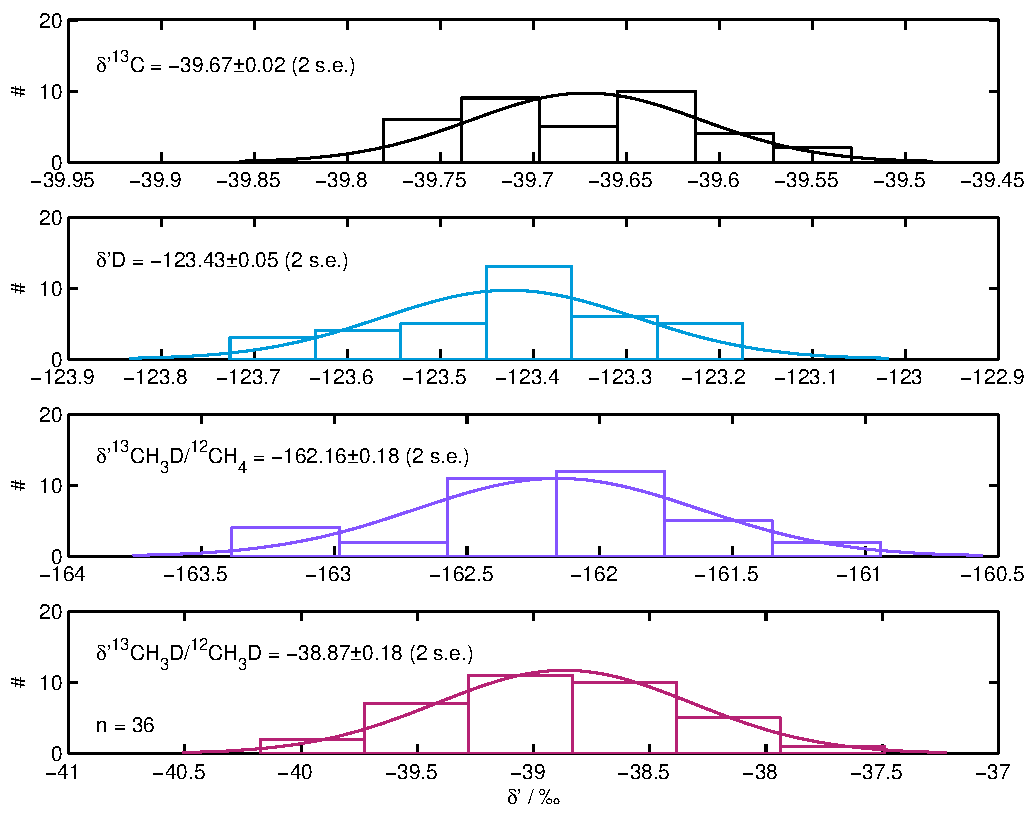
\includegraphics[width=0.85\textwidth]{figures/FigA.3.pdf}
	\captionsetup{format=myformat}	% hrule beneath caption
	\caption[Histogram of isotopologue ratios from a single measurement run]{Histogram of log-delta values (referenced to an
		arbitrary set of isotopologue ratios) for CH\textsubscript{4} purified
		from the Hicks \#1 cylinder, measured on the TILDAS during a single
		sample run (\textasciitilde{}10 hours). Here, \emph{n} represents the
		number of measurement cycles made during this run; in each measurement
		cycle, samples are measured for 100 seconds, and each sample measurement
		is bracketed by measurements on the reference gas.}
	\label{fig:A:3}
\end{figure*}
